\newpage
%%%%%%%%%%%%%%%%%%%%
\section{Animations}
\label{sec:animations}

Sudden and unexpected changes in a user interface, e.g., objects moving from one position to another without any transition between the two states, put a heavy cognitive load on the user, who must mentally relate the states in order to re-assimilate the new display \cite{Chang93}. Animating changes applied to user interface objects transfers part of the user effort to the perceptual level, freeing cognitive processing capacity for application tasks \cite{robertson93}. Aside from the aesthetically pleasant impression it produces on most users when used appropriately, animation therefore contributes to make interfaces more user-friendly.

Animations have been used for didactic purposes, for instance to explain algorithms (see e.g. \cite{carlson96, rodgers00}), but tend to be used more and more just for their above-mentioned ability to reduce the user's cognitive load. For instance, desktop animations are ubiquitous in Apple's Mac OS X and contribute to the perceived quality of this operating system's GUI. Closer to our domain, many information visualization toolkits also support some animation primitives often centered on objects' position. Other toolkits \cite{Chang93, hudson93,bederson00,bederson04} provide more advanced animation support.

ZVTM offers animation capabilities inspired by Stasko's path/transition paradigm \cite{stasko90}. Many user interface changes can be animated following a unified declarative API. Variables to which animations can be applied include:
\begin{itemize}
\item all basic glyph variables (position, orientation, size, color and translucency) and control points of curves (DPath);
\item camera translations and altitude changes (zoom-in/out);
\item magnification lens' radii and magnification factor modifications;
\item portals' location within a view, their size, and translucence.
\end{itemize}

\begin{figure}
\centering
 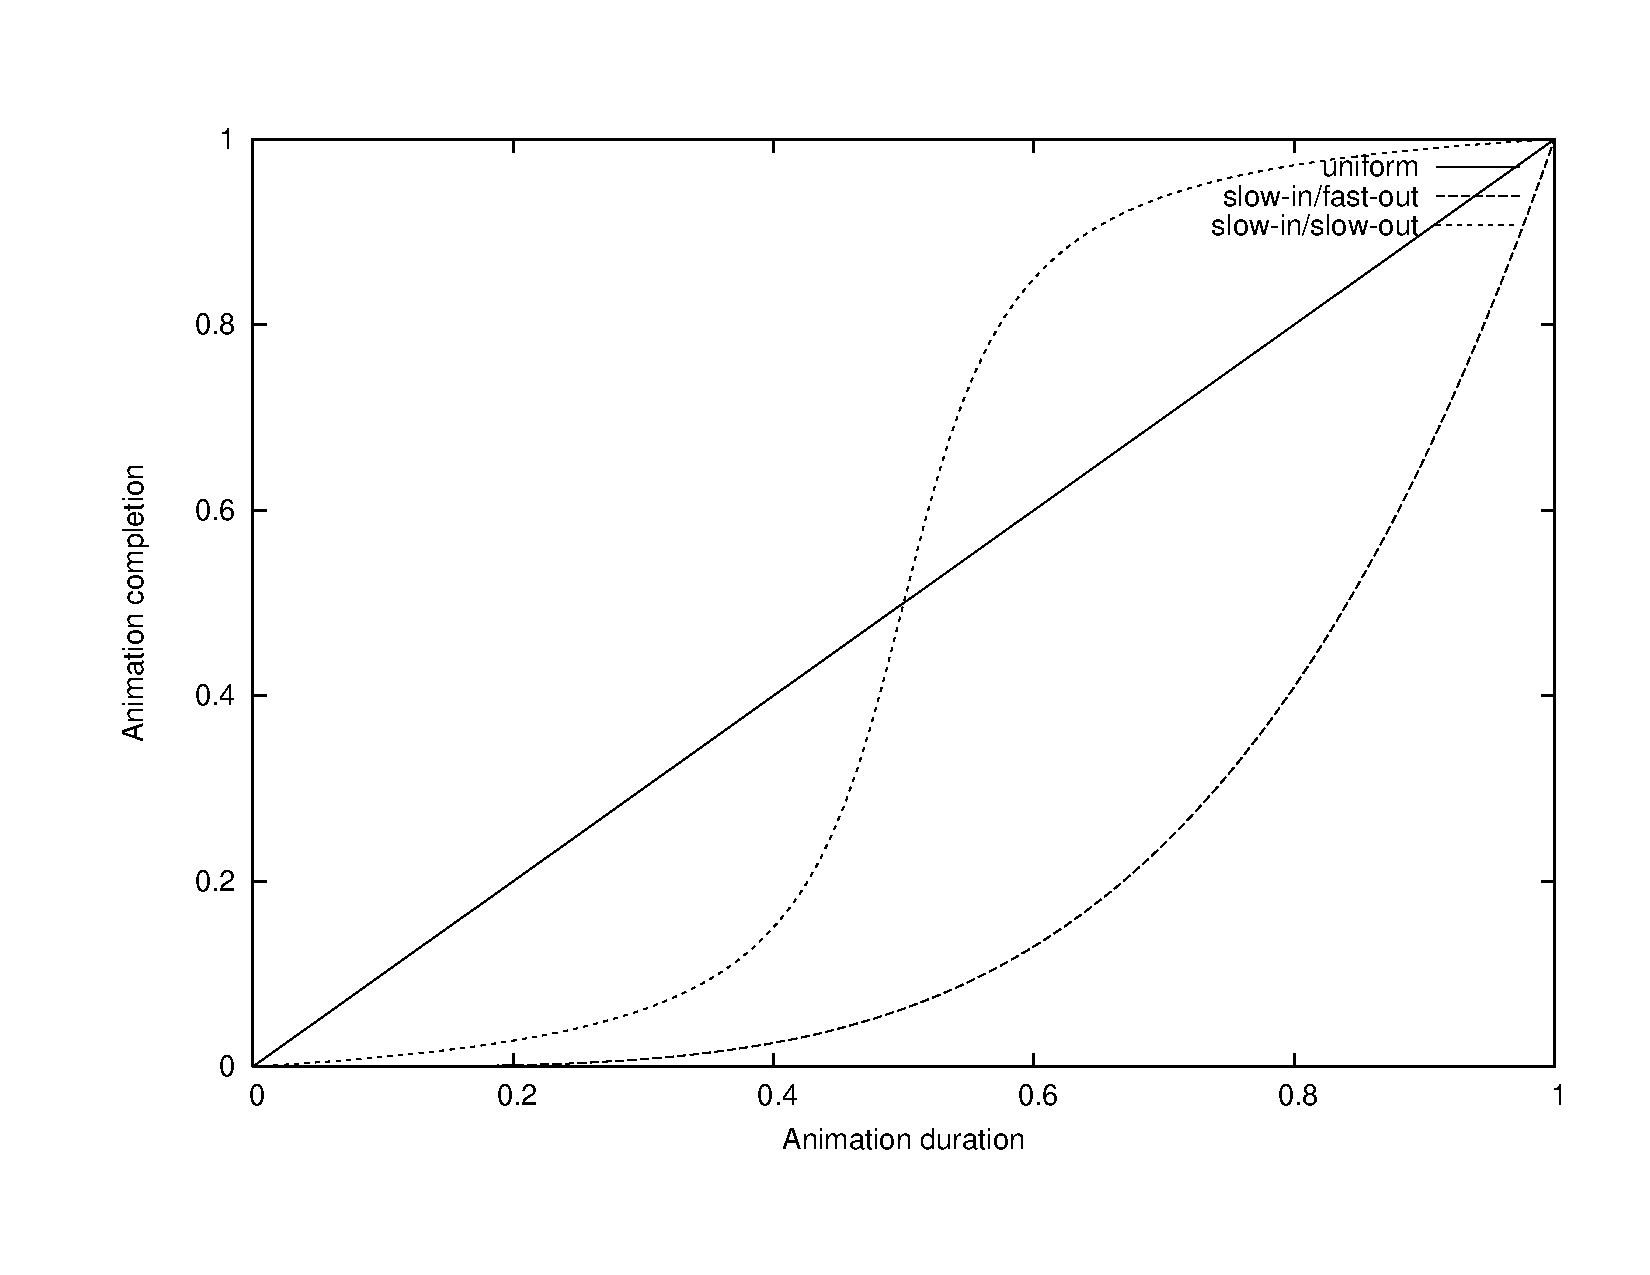
\includegraphics[width=16cm]{images/animSchem.pdf}
  \includegraphics[width=5.5cm,angle=-90]{images/animSchemEx.pdf}
   \caption{Animation pacing functions (top) and example on the translation of a rectangle (bottom)}
   \label{fig:pacing}
\end{figure}

Animations are specified with a single instruction and do not require much more code than the basic modification of a variable's value. They require the following parameters: the animation duration, the object involved, the variable(s) impacted by the animation, the desired target value, and the pacing function. Three off-the-shelf pacing functions are available (Figure \ref{fig:pacing}). Slow-in/slow-out transitions are typically used for camera motion and some glyph animations such as translations, as they convey a feeling of solidity that is important in direct manipulation interfaces \cite{Chang93}. Non-uniform pacing functions are generally used to put emphasis on the start (and/or end) of animation paths. However, they are not always appropriate, and the uniform function is often used when modifying, e.g., magnification lens parameters, or when animating color changes.

Animations are managed by a dedicated thread that controls their timing precisely, skipping steps on the computed animation path if necessary. This mechanism ensures that an animation lasts the specified duration, and runs as smoothly as the system and hardware performance allow. Until v0.9.7, ZVTM was using its own animation engine. Since v0.9.8, the animation engine has been completely rewritten and is now based on Sun's Timing Framework\fref{https://timingframework.dev.java.net/}, and now features additional capabilities in terms of animation management. The use of this more generic API should also make it easy for people already familiar with the Timing Framework to write animations in ZVTM. We only describe the new API in the following.
